\documentclass[12pt]{article}
\title{Time Series Autocorrelation of Key West Yearly Mean Tempertures (1901 - 2000)}
\usepackage{graphicx}
\author{David Scott}
\date{24/10/2018}
\begin{document}
    \maketitle

    \begin{abstract}
        To determine if mean temperature data are significantly correlated with the succesive across time (years) in Key West, Florida. 
        Time series used included data from the year 1901 to 2000. A lag -1 autocorrelation was used and gave a weak r score of 0.326. Random permutated pairs were also 
        generated from the data ten thousand times and tested. This created a random sample to test initial correlation result against. the fraction of these 
        that were greater than intiial correlation was 4e-04. This suggests correlation was non-random. Thus the effect from year to year was significant but weak.  
    \end{abstract} 

    \section{Introduction}
        In class exercise to investigate if mean temperatures from one year are
        significantly correlated with the successive year. 
        Autocorrelation examines data as pairs asseses if a time series is 
        dependent on its past. Pairs of data take form of:
        \begin{equation}
        (x[t],x[t-1]) \  \
        t = observation index. 
        \end{equation}
        Estimated sample correlation of these pairs is the lag -1 autocorrelation. 

    \section{Methodology}
        To calculate the lag -1 autocorrelation, a time series of yearly mean temperatures collected in Key West, 
        Florida from the year 1901 to 2000. This data was imported into RStudio environment. 
        An initial correlation score was calculated using each succesive pair in the sequence. 
        Subsequently repeated calculation ten thousand times by randomly permutating the time series and
        the correlation coefficient was recalculated for each year sequence. Finally the 
        fraction of the ten thousand correlation coefficient that were greater than the 
        initial autocorrelation was calculated as a p value. 

    \section{Results}
        From the initial correlation, an estimated lag-1 autocorrelation
        score of 0.326 was calculated. This is represented by the red 
        abline in figure 1. The autocorrelations generated through 
        the random permutations are displayed as a histogram in figure 1. The fraction of 
        these that were than 0.326 was 4e-04. The abline suggests 
        in figure 1 the intial correlation result falls within the 5% confidence interval. 
        
            \begin{figure}[!h]
            \begin{center}
            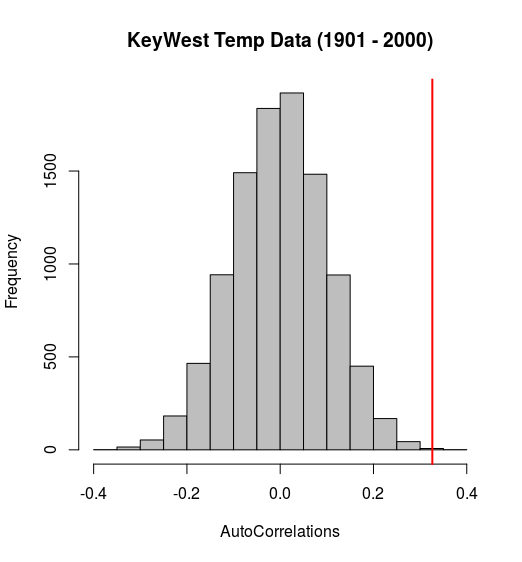
\includegraphics[width=8cm]{../Results/Rplot.png}
            \caption{Frequency of autocorrelations generated from 10,000 random permutations of Key West yearly mean temperature data. 
                Includes abline (red) of autocorrelation of one single correlation of succesive years}
            \end{center}
            \end{figure}

    \section{Discussion}
        In examining figure 1, it is 95\% confident that the first autocorrelation is non-random. 
        This is supported by a significantly low p-value. This suggest that
        the temperature is significantly impacted by the previous year but the impact recorded is weak. 

    \end{document}
